\documentclass{article}
\usepackage[utf8]{inputenc}
\usepackage[T1]{fontenc}
\usepackage{amsmath,enumerate}
\usepackage[thmmarks, amsmath, thref]{ntheorem}
\usepackage{amsfonts}
\usepackage{graphicx}
\usepackage{multicol}
\usepackage{subfig}
\usepackage{float}
\usepackage{tabularx}
\PassOptionsToPackage{hyphens}{url}\usepackage{hyperref}

\title{dialog-de\\Project Report}
\author{}
\date{January 20, 2021}

\begin{document}
\maketitle

\tableofcontents


\section{Introduction}
Dialogue systems are still subject to open research and one might suspect that
deep learning architectures can lead to a better perfomance in this field. The easiest approach would be to
use an unsupervised language model like BERT or GPT-3 as is. This approach is rather limited however, especially
for domain-specific chatbots. A recent paper \cite{wu-xiong-2020-probing} has shown empirically that deep learning models
trained on dialogue data specifically perform better than general-purpose models like BERT and GPT-2. Most of these dialogue-based deep learning models
are only available for the English language, however. Therefore, this project attempts to create a dialogue model suited
for the German language by assembling a German dialogue dataset.


\section{Goal}
There are multiple approaches to chatbots. A common first step of a chatbot is to define \textit{intents} using a set of
utterances. If a user messages a chatbot, the chatbot attempts to detect the intent of the message and responds with a
corresponding hand-coded answer. The dataset for this intent detection has to be manually entered, leading to a relatively small dataset. Hence, intent detection is a few-shot learning task and models trained directly on intent dataset without priors yield insufficient performance. Deep learning could be a solution, since a large
unsupervised language model trained on text data could be finetuned to the small intent detection dataset. In practice, however, this naive approach fails and deep learning models should additionally be pretrained on dialogue data \cite{wu-xiong-2020-probing}. 

This first chatbot step of \textit{intent detection} will serve as demo of this project. The goal is to train a model which
learns dialogue-specific text representations using a dialogue dataset. These representations can then be used for an
intent detection classifier. This classifier can then be evaluated with the F1-score metric similar to \cite{wu-xiong-2020-probing}.

\section{Solution}

\subsection{Model}
The ConveRT model \cite{henderson-etal-2020-convert} was proposed recently and holds the first place in the comparison of \cite{wu-xiong-2020-probing}. The model is pretrained
on English Reddit comments using a response selection task. However, the authors did not provide a reference
implementation and too little information to recreate it. Additionally, they found that ConveRT representations
miss certain language information and have to be complemented with a general purpose language representation \cite{casanueva-etal-2020-efficient}.

Another approach is then to start with a pretrained language model (like BERT), train it on dialogue data using a specific dialogue task and
use the resulting model for dialogue representations. This has been successfully attempted with the TOD-BERT model \cite{wu-etal-2020-tod}.
This model architecture will be used in this project.

\begin{figure}[h]
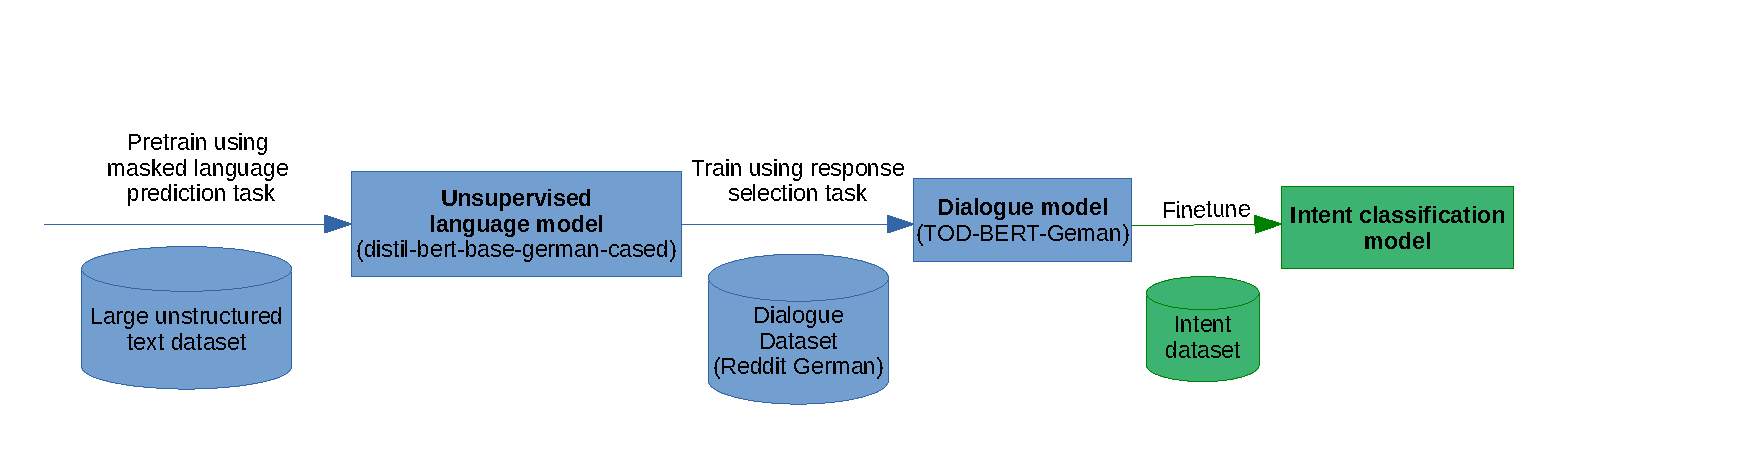
\includegraphics[width=1.2\textwidth]{dialog-arch}
\caption{Architecture summary}
\label{fig:arch}
\end{figure}

\autoref{fig:arch} displays the implemented architecture. distilbert-base-german-cased \footnote{\url{https://huggingface.co/distilbert-base-german-cased}} \cite{distilbert} will be used as pretrained language model. DistilBERT is a smaller version of BERT. This model can be used for sentence embeddings by extracting the embedding for the special \texttt{[CLS]} token inserted at the start of every sentence. However, as has already been established, this sentence embedding is not optimal for dialogue tasks as is. Hence, the model will then be trained on a dialogue dataset using a response selection task. This should lead to robust dialogue representations. The resulting model is called TOD-BERT-German.

The dialogue representations of TOD-BERT-German can then be used for downstream tasks, visualized in green in \autoref{fig:arch}. The downstream task used to demonstrate the dialogue representation is intent classification. An intent classification model can be trained by finetuning the TOD-BERT-German representations on a small intent dataset using the cross-entropy loss. Other examples for downstream tasks include dialogue state tracking, slot-filling, dialogue act prediction etc.

\subsection{Dataset}
The original TOD-BERT model is trained using the MetaLWOz dataset \cite{lee2019multi-domain}. This dataset was manually collected using Mechanical Turk. A similar dataset both in structure as well as in quality is constructed for TOD-BERT-German. In contrast to MetaLWOz however, the dataset is collected automatically due to resource constraints. In this project, this dataset consists of German Reddit conversations. However, the dataset is
structured in a way so that other sources could potentially be added (such as forums, QA sites, IRC threads, e-mail archives, chats, Twitter, etc.). Reddit was used since it covers a diverse range of domains and can be easily scraped. It is obviously not perfect, since discussions are not exclusively task-oriented.

To ensure proper quality, heavy manual heuristics have to be used in the data collection. Reddit discussions are organized in \textit{subreddits}. The Reddit website was scraped for the biggest German subreddits. These subreddits were then used to find other, smaller subreddits manually. A submission to these subreddits could consist of a text post, media or a hyperlink. Only text posts were considered for the dataset. Since submissions can be flaired (i.e. tagged), it is possible to restrict submissions further down to only question-related submissions. Each comment to each text post to which the original poster (OP) responds can then be used as an individual dialogue, with the dialogue turns consisting of the comment-reponse chain.

\begin{verbatim}
{
	"domain": "subreddit",
	"initialIntent": "flair",
	"title": "submission title",
	"id": "aaaaaa",
	"turns": [
		{
			"sender": "user",
			"text": "question"
		},
		{
			"sender": "sys",
			"text": "response"
		}
	]
}
\end{verbatim}

The listing above shows an example record of the data. The record includes the submission title and id. The flair is used as a loose approximation of initial intent if available and the subreddit name is used as domain. These metadata are not used down the line but may be useful for other purposes. The OP is designated as the human user the dialogue, while the poster responding to OP is designated as the system response which a dialogue system should be able to emulate. This situation is inverted for the special type of \textit{AmA} (Ask me Anything) submissions, which solicit questions in the comments.

A range of indications are used to ignore texts. For example, Reddit users often denote sarcasm using \texttt{\textbackslash s}. These texts are ignored. Additionally, every text containing hyperlinks or bot commands is ignored for obvious reasons. Furthermore, the score (i.e. the difference between upvotes and downvotes) is used as a rough quality heuristic. Submissions or comments with negative scores are ignored.

The dataset is constructed by scraping the respective Reddit websites. The script is paralellized and attempts to use as little HTTP requests as possible. Overall, gathering the data takes around a day. The 30MB dataset contains 7619 dialogues. Further statistics are displayed in \autoref{tab:stats}.

\begin{table}
\begin{tabular}{c r r r r}
Statistic & Min & Mean & St dev & Min \\
\hline
Turns per dialogue & 2 & 12.58 & 11.93 & 79 \\
Turn lengths & 1 & 267.39 & 389.42 & 9183 \\
Words per turn & 1 & 42.58 & 60.84 & 1415
\end{tabular}
\caption{Dataset statistics}
\label{tab:stats}
\end{table}

Texts longer than 512 tokens are not used to train the model, similar to other work (e.g. ConveRT uses only texts with 9 to 128 words).

\subsection{Results}
The TOD-BERT-German models are trained using a combination of the Masked Language Modelling and the Response Selection loss. Both this loss and the perplexity can be used to compare models trained using different configurations. In the end, three configurations made a difference, as can be seen in \autoref{tab:tod}. The first model is trained using the default configuration. Adding weight decay or a different learning rate did not change the result. Training the model using automatic mixed precision (amp) lead to improved metrics. Choosing negative samples for the response selection tasks using k-means improved the metrics even further. It is important to note that is hard to accurately measure model performance (especially wrt downstream tasks) using the loss and perplexity alone. In practice, results in the downstream task (intent classification) were virtually the same for the three configurations. Due to the excessive time needed to train the models, additional configurations were not tried. It is very likely that a more optimal model could still be found.

\begin{table}
	\begin{tabular}{l r r r}
	Model & Loss & Perplexity & Steps until convergence \\
	\hline
	default & 0.725 & 2.066 & 310,000 \\
	amp & 0.743 & 1.996 & 225,000 \\
	kmeans + amp & \textbf{0.691} & \textbf{1.988} & 400,000 \\
	\end{tabular}
\caption{Comparison of TOD-BERT-German configurations}
\label{tab:tod}
\end{table}

The resulting TOD-BERT-German model can then be finetuned on an intent dataset and compared to other intent classification models. The Rasa framework\footnote{\url{https://github.com/rasahq/rasa}} is used to setup a chatbot. The intent data is adapted from \url{https://github.com/zdi-mainfranken/corona-chatbot}. TOD-Bert-German is compared to the default intent classification pipeline in Rasa (DIET, based on bag of words and Transformers) and to a pipeline based on Spacy word vectors (using \texttt{de\_core\_news\_md}\footnote{\url{https://spacy.io/models/de/}}). \autoref{tab:intent} shows the F1-score of each model based on 5-fold cross validation. It can be seen that TOD-BERT-German outperforms both DIET and Spacy by a small margin. While this difference remains consistent across multiple runs, it is by no means extreme.

\begin{table}
	\begin{tabular}{l r}
		Model & F1-score \\
		\hline
		TOD-BERT-German & \textbf{0.642} \\
		DIET & 0.626 \\
		Spacy & 0.614 \\
	\end{tabular}
\caption{Comparison of different models on intent classification}
\label{tab:intent}
\end{table}

\section{Discussion}

Limitations of this work include that the dataset consisting of German Reddit texts only is obviously just a beginning. It should be complemented with data from other websites in order to increase the diversity and to prevent the model from overfitting to Reddit-style messages.

The tokenization used (Distil)BERT is optimized for the English language. Ideally, a BERT-like model for the German language would use a different tokenization procedure. Training such a model requires a lot of resources however, and the available pretrained models use the original tokenizer. In the same vein, the chosen DistilBERT model was distilled using a BERT model which was trained on an older version of the training code. That means that this model does not include the recent Whole Word Masking bugfix\footnote{\url{https://github.com/google-research/bert/commit/0fce551b55caabcfba52c61e18f34b541aef186a}}.

There are also different language models available that could be used in this architecture (e.g. GPT-2). The only reason BERT was chosen was because a distilled version (DistilBERT) was available.

The main lesson learnt during this project is that when face with time constraints it is preferrable to start with a simple, achievable idea. Additionally, it is advisable to use Docker containers instead of trying to setup the dependencies on the host, since this is an error-prone process. Also, resolving the discrepancy between research code (using Pytorch and CUDA 11) and the deplyoment with Rasa (using an older version of Tensorflow) was time-consuming and educational. If possible it is advisable to stick to one framework and version for a new project.


The time spent on specific tasks can be viewed in \autoref{tab:times}.
\begin{table}
\begin{tabular}{c r}
Task & Hours \\
\hline
Dataset creation & 25 \\
Training the network & 20 \\
Building the application & 15 \\
Writing the final report & 5 \\
Preparing the presentation of your work & 8 \\
\end{tabular}
\caption{Work breakdown}
\label{tab:times}
\end{table}


\bibliographystyle{plain}
\bibliography{report}

\end{document}
